\chapter{Concentration and Martingales}
	
	At the moment, we have seen that randomised algorithms can dramatically increase the 
	efficiency with which a problm may be solved, if we are willing to accept a certain error, 
	and a certain degree of uncertainty about even the large picture of how the algorithm will 
	run, which is clearly a disadvantage when comparing to deterministic algorithms, which are 
	totally predictable, of course. 
	\\
	There is a property of random variables that essentially measures how close the variables 
	remain to their expected value; this property is known as \emph{concentration}. Clearly, 
	if we can dervie randomised algorithms with a high concentration we my be able to harness 
	the benefits of randomisation whilst staing close to determinism, which would be 
	advantageous. This chapter discusses firstly how we may work with concentration, and 
	derive probaility bounds for it, known as \emph{concentration inequalities}.
	\section{Concentration Inequalities}
	Recall the First- and Second-Moment methods (the Markov and Chebyshev inequalities, 
	respectively) of Chapter 1:
	\begin{reptheorem}{theorem:markovineq}[Markov Inequality]
		Let $X$ be a random variable with nonnegative range, and let $a \in \mathbb{R}^+$.
		Then 
		$$
			\mathbb{P}(X \geq a) \leq \sfrac{\mathbb{E}(X)}{a}.
		$$
	\end{reptheorem}
	\begin{reptheorem}{theorem:chebineq}[Chebyshev Inequality]
		Let $X$ be some random variable, and let $a\in \mathbb{R}^+$. Then
		$$
			\mathbb{P}(|X-\mathbb{E}(X)| \geq a) \leq \sfrac{\mathrm{var}(X)}{a^2} 
		$$
	\end{reptheorem}
	\begin{comment}
		From the Markov inequality, we can obtain the two following results, too, where 
		$f \in \mathbb{R}\rightarrow 0,\infty)$:
		\begin{enumerate}[(1)]
			\item
			If $f$ is an increasing function, then 
			$$
			\mathbb{P}(X \geq a) \leq \mathbb{P}(f(X) \geq f(a)) \leq 
			\sfrac{\mathbb{E}(f(X))}{f(a)}.
			$$
			\item
			If $f$ is a decreasing function, then 
			$$
			\mathbb{P}(X \leq a) \leq \mathbb{P}(f(X) \geq f(a)) \leq 
			\sfrac{\mathbb{E}(f(X))}{f(a)}.
			$$
		\end{enumerate}
		We will soon see that using these, and choosing appropriate functions, we may 
		obtain significantly tighter concentration inequalities than the classical Markov 
		and Chebyshev bounds, in the sense explained by the following example.
	\end{comment}

	Consider the experiment in which $n$ coins with probability $p$ of turning up heads are 
	thrown independently, then if $n$ grows large the number of heads should be around $p\cdot 
	n$. We can try to justify this with the Markov and Chebyshev inequalities---let $q 
	\coloneqq 1-p$, and let $d \in \mathbb{R}^+$ be a fixed constant, and let $X$ be the 
	number of heads thrown in the experiment. Then
	\begin{itemize}
		\item By the Markov inequality,
		\begin{align}
			\nonumber
			\mathbb{P}(X \geq (1+\delta)pn) &\leq \frac{\mathbb{E}(X)}{(1+\delta)pn} \\
			&= \frac{pn}{(1+\delta)pn} \nonumber \\
			&= \frac{1}{1+\delta} \label{badmarkovbound}.
		\end{align}
		This bound is bad, since it gives the same probability bound for any $n$, which is 
		useless in practice.
		\item By the Chebyshev inequality, however,
		\begin{align}
			\nonumber
			\mathbb{P}(|X-pn|\geq\delta pn)&\leq\frac{\mathrm{var}(X)}{\delta^2p^2n^2}\\
			&= \frac{pqn}{\delta^2p^2n^2} \nonumber\\
			&= \frac{1-p}{\delta^2pn} \label{betterchebbound}
		\end{align}
		Which tends to 0 as $n$ grows large, meaning that this is a much better bound on 
		the concentration. However, it tends to zero only with linear speed, which, as we 
		shall see, can yet be improved upon dramatically.
	\end{itemize}
	The Markov and Chebyshev inequalities make use of the first and second moments. Using the 
	moment-generating function from Section 1.2.2, we will take more moments to derive the 
	so-called \emph{Chernoff bounds}.

	\subsection{Introduction to Chernoff Bounds}
	So recall the moment-gnerating function introduced in Chapter 1; for a random variable $X$
	it is $M_X(t) \coloneqq \mathbb{E}(\exp(tX))$. We will see that the parameterisation 
	of this function on $t$ will be useful: For any $t > 0$, we have that 
	$$
		\mathbb{P}(X\geq a)=
		\mathbb{P}(e^{tx}\geq e^{ta})\leq\exp(-ta)\cdot\mathbb{E}(\exp(tX)).
	$$
	Therefore, in particular, 
	$$
		\mathbb{P}(X\geq a)\leq\min_{t>0}(\exp(-ta)\mathbb{E}(\exp(tX))).
	$$
	Of course, we can similarly obtain that 
	$$
		\mathbb{P}(X\leq a)\leq\min_{t<0}(\exp(-ta)\mathbb{E}(\exp(tX))).
	$$
	Where the equality in the first equation holds because $\exp$ is injective. We shall see
	how to chose appropriate values for $t$ to derive useful concentration inequalities; and 
	that, even though the values of $t$ that minimise the above expressions provide the 
	tightest bounds, it is often preferable to chose other values of $t$ that make for more 
	convenient bounds to work with. \par

	So let us come back to our example of flipping $n$ coins, but let us make the example 
	slightly more general, and allow each coin to have a different bias, so that coin $X_i$ has 
	probability of turning up heads $p_i$ (aside: Each coin is a \emph{Poisson trial}, which 
	differs from a Poisson distribution, and is a more general case of a sequence of Bernoulli 
	trials). Then, let $X \coloneqq \sum_i X_i$, and denote $\mu \coloneqq \mathbb{E}(X) = 
	\sum_i p_i$.\par

	We will develop Chernoff bounds corresponding to the bound presented in 
	(\ref{badmarkovbound}), for which we shall need to develop the mgf for $X$. Beginning with 
	the mgfs for the individual $X_i$, we have that
	\begin{align*}
		M_{X_i}(t) &= \mathbb{E}(\exp(tX_i)) \\
		&= p_i e^t + (1-p_i)\\
		&= 1 + p_i (e^t-1) \\
		&\leq \exp(e^t - 1) & \text{since $\forall x. 1+x \leq e^x$.}
	\end{align*}
	We can now apply theorem \ref{theorem:summgf} to obtain the mgf of $X$, since each of the 
	coins is thrown independently from the others. That is, 
	\begin{align*}
		M_X(t) &= M_{\sum X_i} \\
		&= \prod_{i=1}^{i=n} M_{X_i} \\
		&\leq \prod_{i=1}^{i=n} \exp{p_i(e^t- 1)} \\
		&=\exp\left(\sum_{i=1}^{i=n}p_i(e^t - 1)\right) \\
		&=\exp(\mu \cdot (e^t- 1))
	\end{align*}

	We can now present the Chernoff bounds for the sum of $n$ indpendent coin flips, as stated
	in theorem \ref{theorem:chernoff}.
	\begin{theorem}
		\label{theorem:chernoff}
		Let $X_1\hdots X_n$ be independent Poisson trials with parameters $p_1\hdots p_n$.
		Let $X = \sum_{i=1}^{i=n} X_i$ and $\mu = \mathbb{E}X$. Then the following bounds 
		hold:
		\begin{enumerate}
			\item For any $\delta > 0$, 
			\begin{align}
				\mathbb{P}(X \geq (1+\delta)\mu) \leq 
				\left(\frac{e^\delta}{(1+\delta)^{(1+\delta)}}\right)^\mu.
				\label{chernoff1}
			\end{align}
			\item For any $\nu > \mu$, 
			\begin{align}
				\mathbb{P}(X \geq \nu) \leq e^{-\mu} \left(e\mu\nu^{-1}\right)^\nu
				\label{altchernoff1}
			\end{align}
			\item For any $\epsilon > 0$,
			\begin{align}
				\mathbb{P}(X\geq \mu+\epsilon)\leq\exp(-2\sfrac{\epsilon^2}{n}).
				\label{altchernoff2}
			\end{align}
			\item For any $\delta \in (0,1)$,
			\begin{align}
				\mathbb{P}(X\geq (1+\delta)\mu) \leq \exp(-\mu\sfrac{\delta^2}{3}).
				\label{chernoff2}
			\end{align}
			\item For any $R \geq 6\mu$,
			\begin{align}
				\label{chernoff3}
				\mathbb{P}(X\geq R) \leq 2^{-R}
			\end{align}
		\end{enumerate}
	\end{theorem}
	
	Before we prove these bounds, we shall consider the theorem's implications for the example 
	we had considered earlier, where all coins share parameter $p$. 
	\\
	The Chernoff bound presented in equation (\ref{chernoff1}) means that, for $n$ coins with 
	bias $p$, the total number $X$ of heads satisfies 
	$$
		\mathbb{P}(X \geq (1+\delta)pn) \leq
		\left(\frac{e^\delta}{(1+\delta)^{(1+\delta)}}\right)^{pn}
	$$
	which is clearly an \emph{exponentially} better bound on the probability than that 
	presented in equation (\ref{badmarkovbound}) for a fixed $\delta >0$ as $n$ grows large.
	\\
	To illustrate this with an example, consider the case when $p = \sfrac{1}{2}$ and $n=100$.
	We wish to bound the probability that at least 75 coins come up heads, that is $X \geq 75 =
	\sfrac{3}{2} \cdot \mu$. 
	\begin{itemize}
		\item By Markov's inequality, we can bound this probability as $\mathbb{P}(X \geq 
		\sfrac{3}{2} \mathbb{E}(X)) \leq \sfrac{2}{3} \approx 0.667$. We could have guessed
		as much.
		\item Chebyshev's inequality, however, allows us to bound the probability as 
		\begin{align*}
			\mathbb{P}(X \geq \mathbb{E}(X) + 25) &= 
			\sfrac{1}{2} \mathbb{P}(|X-\mathbb{E}(X)| \geq 25) & \text{by the symmetry 
			of the binomial distribution}\\
			&\leq \frac{\mathrm{var}(X)}{2 \cdot 25^2} \\
			&= \sfrac{1}{50} = 0.02,
		\end{align*}
		which is clearly a much tighter bound.
		\item Finally, the Chernoff bound as stated in equation (\ref{chernoff1}) bounds 
		this probability as 
		\begin{align*}
			\mathbb{P}(X \geq \sfrac{3}{2} \mathbb{E}(X)) &\leq 
			\left(\frac{e^{\sfrac{1}{2}}}{(\sfrac{3}{2})^{\sfrac{3}{2}}}\right)^{50} \\
			&\approx 0.004472
		\end{align*}
		which is, yet again, a full order of magnitude better. Calculating the probability 
		explicitly gives it as roughly $\num{2.8e-7}$. This example shows us the power of 
		Chernoff bounds; it should be kept in mind, however, that these Chernoff bounds 
		require the individual random variables $X_i$ to be independent of one another, 
		which the Markov and Chebyshev inequalities do not. 
	\end{itemize}

	We shall also consider a second example; we revisit that of throwing $m$ balls into $n$ 
	bins, discussed previously. For now, we consider a singular bin; we would like to consider 
	the maximum load on a single bin, say $b$.\\
	Therefore, let $X_i$ be the indicator random variable of ball $i$ going into $b$, and let $
	X = \sum_{i=0}^{i=m} X_i$. Thus, each of the $X_i$ is a Poisson trial with parameter $p_i 
	= n^{-1}$. Now, if we set $m = 2n \cdot \ln n$, then $\mu = \mathbb{E}(X) = 2 \cdot \ln n$, 
	and so, by the Chernoff bound of equation (\ref{altchernoff1}) we have 
	\begin{align*}
		\mathbb{P}(X \geq 6\cdot\ln n) &\leq 
		\exp(-2\ln n)\left(\frac{2e \ln n}{6 \ln n}\right)^{6n \dot\ln n} \\
		&\leq \exp(-2 \ln n) \\
		&= n^{-2}
	\end{align*}
	So let $\mathcal{E}_b$ be the event that bin $b$ receives at least $6 \cdot \ln n$ balls.
	We care about the event that \emph{at least one} bin does, that is, we care about the 
	event $\mathcal{E} \coloneqq \bigcup_{b=1}^{b=n} \mathcal{E}_b$. \\
	We use the union bound to establish that $\mathbb{P}(\mathcal{E}) \leq \sum_{b = 1}^{b=n} 
	\mathbb{P}(\mathcal{E}_b) \leq n^{-1}$. That is, the event that no bin receives at least 
	$6 \ln n$ balls occurs \emph{with high probability}! Now, at the moment, the choice of $6 
	\ln n$ balls upper bound as being of interest may seem slightly arbitrary. However, we 
	draw attention to the fact that, by the pigeon-hole principle, at least one bin receives at 
	least $2 \ln n$ balls when throwing $m = 2n\cdot \ln n$ balls in total. So we established 
	that the maximum load under this value for $m$ is $\Theta(\log n)$. \\
	We compare this with the case where $m=n$. Again, by using the Chernoff bound presented in 
	equation (\ref{altchernoff1}), we get
	$$
		\mathbb{P}(X>\nu) \leq e^{-1} \left(\sfrac{e}{\nu}\right)^\nu \leq 
		\left(\sfrac{e}{\nu}\right)^\nu
	$$
	So consider the case where $\nu = 4 \frac{\ln n}{\ln(\ln n)}$, where we thus obtain 
	$\mathbb{P}(X > \nu) \leq n^{-2}$ if $n$ is large enough, since 
	\begin{align}
	\nonumber
		\left(\sfrac{e}{\nu}\right)^\nu &= \exp\left(\frac{4\ln n}{\ln\ln n} \cdot 
		\ln\left(\frac{e\ln(\ln n)}{4 \ln n}\right)\right) \\
		\intertext{where the term inside the exponential is}
		\nonumber
		\frac{4\ln n}{\ln(\ln n)} \cdot \ln\left(\frac{e\ln(\ln n)}{4 \ln n}\right) &=
		\frac{4\ln n}{\ln(\ln n)} \cdot (\ln(\sfrac{4}{e}) + \ln\ln\ln n - \ln\ln n) \\
		\label{stepwithlargen}
		&\leq \frac{4\ln n}{\ln(\ln n)} \cdot (-\sfrac{1}{2} \ln\ln n) \\
		\intertext{from which it follows that}
		\mathbb{P}(X> \nu) &\leq n^{-2}
	\end{align}
	where step (\ref{stepwithlargen}) only holds for sufficiently large $n$. \\
	Thus, with high probability, by the union bound, the maximum load when $m=n$ is of order 
	$O\left(\frac{\log n}{\log \log n}\right)$. However, it can be shown that with high 
	probability, at least one bin does receive $\Omega\left(\frac{\log n}{\log \log n}\right)$
	balls, meaning that, wven though the expected value of balls each bin should receive is 
	$1$, the maximum load is expected to be much larger. 
	\\
	We can thus conlcude that, when we have $m \in O(n \cdot \log n)$, the method of simply 
	randomly assigning balls to bins is ``good'', in that the maximum load is almost surely 
	the expected number of balls each bin should receive (within a constant factor), while the 
	algorithm is ``bad'' in the same sense when $m \in O(n)$.
	\\
	It is actually possible to improve the performance of this algorithm with a very simple 
	modification, by employing a techique known as the \emph{pwer of two choices}: If, instead 
	of sampling one bin at random for each ball, we sample two, and assign the ball to the bin 
	with lower load, then it can be shown that, with high probability, the maximum load will 
	be $\Theta(\ln\ln n)$.
	\par
	We will now proceed to prove the Chernoff bounds presented in theorem 
	\ref{theorem:chernoff}, with the exception of the bound presented in equation 
	(\ref{altchernoff2}), the proof of which we delegate to a later section.
	\begin{proof}[Proof of theorem \ref{theorem:chernoff}]
		Recall the result which we had previously established: $\forall t. M_X(t) \leq 
		\exp(\mu(e^t-1))$. Thus we may apply Markov's inequality to obtain
		\begin{align*}
			\mathbb{P}(X\geq(1+\delta)\mu) &=\mathbb{P}(e^{tX}\geq e^{t(1+\delta)\mu})
			\\
			&\leq \frac{\mathbb{E}(e^{tX})}{\exp(t(1+\delta)\mu)}\\
			&\leq \frac{\exp\left(\left(e^t-1\right)\mu\right)}{\exp(t(1+\delta)\mu)}
		\end{align*}
		Which reduces to equation \ref{chernoff1} when we set $t = \ln(1+\delta)$. \\
		Having derived this equation, it is straightforward to conclude equation 
		\ref{altchernoff1} by setting $\nu = (1+\delta) \mu$, which satisfies the conditon 
		that $\nu > \mu$ since $\delta > 0$.\\
		To prove the the equation (\ref{chernoff2}), it will suffice to show that for 
		$\delta \in (0,1)$, 
		$$
			\left(\frac{e^\delta}{(1+\delta)^{(1+\delta)}}\right)^\mu \leq
			\exp(-\mu\sfrac{\delta^2}{3}).
		$$
		An equivalent condition is obtained by taking logarithms on both sides, so let 
		$$
			\Delta \coloneqq \lambda \delta\ .\  
			\delta - (1+\delta) \ln (1+\delta) +\sfrac{\delta^2}{3}
		$$
		and note that we may prove the equation (\ref{chernoff2}) if we can show that 
		$\forall \delta\in (0,1). \Delta(\delta) \leq 0$.\\
		To this end, note that $\Delta(0) = 0$, and $\Delta(1) = \sfrac{4}{3} - 2\ln 2 <0$.
		Then, denote 
		$$
			\Delta' \coloneqq \frac{\mathrm{d}\Delta}{\mathrm{d}\delta} = 
			1 - \ln(1+\delta) - \frac{1+\delta}{1+\delta} +\sfrac{2}{3} \delta = 
			\sfrac{2}{3} \delta - \ln(1+\delta)
		$$
		and
		$$		
			\Delta'' \coloneqq \frac{\mathrm{d}^2\Delta}{\mathrm{d}\delta^2} = 
			\sfrac{2}{3} - (1+\delta)^{-1}
		$$
		Then note that $\Delta'(0) = 0 \land \Delta''(0) < 0$, with $\Delta''(\delta) = 0 
		\implies \delta=\sfrac{1}{2}$. These imply that the dunction $\Delta$ decreases for 
		$\delta$ close to $0$, andthe speed at which it decreases grows until $\delta=
		\sfrac{1}{2}$, at which point the speed of the decrease of $\Delta$ slows down.
		However, note that $\Delta'(1) < 0$, meaning that $\forall \delta \in (0,1). 
		\Delta(\delta) < 0$, so equation (\ref{chernoff2}) holds. \\
		Finally, suppose $\delta > 5$ and let $R \coloneqq (1+\delta)\mu$, so 
		\begin{align*}
			\mathbb{P}(X \geq R) &\leq 
			\left(\frac{e^\delta}{(1+\delta)^{(1+\delta)}}\right)^\mu \\
			&\leq \left(\frac{e}{(1+\delta)}\right)^{(1+\delta)\mu} \\
			&\leq \left(\frac{e}{6}\right)^R \\
			&\leq 2^{-R}
		\end{align*}
		which conlcudes the proof of equation (\ref{chernoff3}), and so that of the 
		theorem.
	\end{proof}

	Theorem \ref{theorem:chernoff} gives bounds on the upper tail probability of the 
	distribution. We can obtain very similar results  for the lower tail, as collected in 
	theorem \ref{theorem:chernofflower}.
	\begin{theorem}
		\label{theorem:chernofflower}
		Let $X_1\hdots X_n$ be independent Poisson trials with parameters $p_1\hdots p_n$.
		Let $X = \sum_{i=1}^{i=n} X_i$ and $\mu = \mathbb{E}X$. Then the following bounds 
		hold:
		\begin{enumerate}
			\item For any $\delta \in (0, 1)$, 
			\begin{align}
				\mathbb{P}(X \leq (1-\delta)\mu) \leq 
				\left(\frac{e^{-\delta}}{(1-\delta)^{(1-\delta)}}\right)^\mu.
				\label{chernofflower1}
			\end{align}
			\item For any $\nu < \mu$, 
			\begin{align}
				\mathbb{P}(X \leq \nu) \leq e^{-\mu} \left(e\mu\nu^{-1}\right)^\nu
				\label{altchernofflower1}
			\end{align}
			\item For any $\epsilon > 0$,
			\begin{align}
				\mathbb{P}(X\leq \mu-\epsilon)\leq\exp(-2\sfrac{\epsilon^2}{n}).
				\label{altchernofflower2}
			\end{align}
			\item For any $\delta \in (0,1)$,
			\begin{align}
				\mathbb{P}(X\leq (1-\delta)\mu) \leq \exp(-\mu\sfrac{\delta^2}{2}).
				\label{chernofflower2}
			\end{align}
		\end{enumerate}
	\end{theorem}
	The proof of theorem \ref{theorem:chernofflower} is very similar to that of theroem 
	\ref{theorem:chernoff}, so it is omitted here. It should be noted that the equations 
	(\ref{chernoff2}) and (\ref{chernoff3}) are weaker bounds than equation (\ref{chernoff1}),
	though \emph{arguably} more readable. However, the equation (\ref{altchernoff2}) is 
	actually a \emph{much tighter} bound than that of equation (\ref{chernoff1})\footnote{This 
	is the case because equation (\ref{altchernoff2}) is derived from Hoeffding's Lemma, which 
	we introduce at a later time.} for sufficiently large $\mu$ in proportion to $n$: If $\mu 
	\geq \sfrac{n}{2}$, then 
	$$
		\left(\frac{e^\delta}{(1+\delta)^{(1+\delta)}}\right)^\mu \geq 
		\exp\left(-2\delta^2\mu^2n^{-1}\right),
	$$
	where we can obtain the result from setting $\epsilon = \delta\mu$. Analogous facts hold 
	for the equations in theorem \ref{theorem:chernofflower}.
	\\
	It may also be relevant to note that, from equations (\ref{chernoff2}) and 
	(\ref{chernofflower2}), we may obtain yet another alternative form of the Chernoff bound, 
	as described in lemma \ref{lemma:relchernoff}.
	\begin{lemma}
	\label{lemma:relchernoff}
		If $X$ is the sum of $n$ Poisson trials $X_i$, then
		$$
			\forall \delta \in (0,1)\ .\ \mathbb{P}(|X - \mu| \geq \delta\mu) \leq
			2 \exp(-\sfrac{\delta^2}{3}).
		$$
	\end{lemma}
	
	It may now be worth extracting from this example a brief conclusion of this section, a 
	method we shall call the ``Chernoff technique'' for deriving concentration results for 
	some general random variable.\\
	The general procedure to follow when deriving Chernoff bounds, as illustrated by the proof 
	of theorem \ref{theorem:chernoff}, is the following:
	\begin{enumerate}[(1)]
		\item Use Markov's or Chebyshev's inequality to derive an upper bound on the 
		probability that a random variable deviates from its mean, depending on the random 
		variable's moment-generating function.
		\item Derive an upper bound for the moment-generating function $M_X(t)$.
		\item Optimize this with respect to $t$ to determine the tightest bound.
	\end{enumerate}

	\subsection{Application: QuickSort}
	The last thing we shall consider in this brief introduction to Chernoff bounds is how they 
	relate to one of the most well-known algorithms we have already encountered; QuickSort. Of 
	course, the standard implementation of QuickSort is not a randomised algorithm, but we 
	also know of any easy extension to the algorithm that introduces randomisation and removes 
	the one great vulneability of the algorithm.\\
	Normally, QuickSort suffers quadratic complexity when operating on a pr{\ae}sorted list.
	By choosing the pivot at random, at each step, however, eliminates this possibility with 
	high probability, as should be reasonably intuitive.\\
	We will consider the complexity of QuickSort as entirely based on the number of 
	comparisons made during the execution of the algorithm, but first let us consider a 
	particular way of modelling the execution of QuickSort on a particular list of numbers. To 
	this end, we choose to represent such an execution as a tree in which each node represents 
	a number that has been chosen as pivot, its subtrees representing the sublists containing 
	the larger, and smaller numbers in the list repsectively. For example, consider the 
	following tree that illustrates the principle:
	\begin{center}
		\Tree 
		[. {[2, 8, 9, 1, 7, 5, \underline{6}, 3, 4]}
			[. {[\underline{2}, 1, 5, 3, 4]}
				[. {[\underline{1}]} ]
				[. [5,3,\underline{4}]
					[. {[\underline{3}]} ]
					[. {[\underline{5}]} ]
				]
			]
			[. {[\underline{9},8,7]}
				[. {[\underline{8}, 7]}
					[. {[\underline{7}]} ]
				]
			]
		]
	\end{center}
	where at each node the underlined number is the chosen pivot. Now note that, a node at 
	depth $l$ has been compared to $l$ different pivots so far, meaning that the sum of the 
	depths of the nodes will be the total number of comparisons made during the execution of 
	the algorithm. In the case of our example, there are three nodes at depths 2 and 3, 
	respectively, 2 at depth 1, and 1 root. This co\"incides with the number of comparisons 
	made, 17.
	\\
	Having established this view of QuickSort, we return to our formal analysis of the 
	algorithm using random pivots. Consider a list of $n$ distinct numbers, and suppose without 
	loss of generality that these numbers are $\{1\hdots n\}$. Consider the execution tree of 
	QuickSort on some permutation of these numbers, and let $L_i$ denote the depth at which $i$
	is chosen as the pivot, then as discussed above, we have $C = \sum_{i=0}^{i=n} L_i$, where 
	$C$ is the number of comparisons made. We shall prove the following result:
	$$
		\exists D \in \mathbb{R} . \mathbb{P}(\forall i. L_i \leq D \log n) \geq 1 - n^{-1},
	$$
	by proving the slightly easier result that each of the leaves is at most at depth $D\log 
	n$, which gives us the result (ie.\ the expected running time of QuickSort as $O(n\log 
	n)$) we know and love (with high probability), formalising the claim we had made earlier. 

	\begin{theorem}
		\label{theorem:quicksortheight}
		If $P$ is a path in the execution tree of random-pivot QuickSort that leads from 
		the root node to a leaf that has ben chosen at random from all such paths, then 
		$\exists D. \mathbb{P}(|P| \leq D \log n) \geq  n^{-1}$.
	\end{theorem}
	\begin{proof}
		Let us call a node of the tree ``bad'' if either one of the sublists represented 
		by the branches of the node is shorter than $\sfrac{1}{3}$ of the length of the 
		list at that node, that is, if the split produced by the pivot chosen is more 
		unbalanced than a $\sfrac{1}{3}$-$\sfrac{2}{3}$ split. Call the node ``good'' 
		otherwise. Further denote by $s_l$ the size of the list at depth $l$ of the path 
		$P$. Then note that, if the node at depth $l$ in $t$ is good, then $s_{l+1} \leq 
		\sfrac{2}{3}$. Hence, the path $P$ can at most contain $\log_{\sfrac{2}{3}}(n) = 
		\frac{\log n}{\ln \sfrac{2}{3}} \leq 2 \ln n$ good nodes. 
		\\
		Fix now $D = 21$, and suppose that $|P| > D \ln n$. Note that this implies that 
		there are more than $19 \ln n$ bad vertices on the path $P$. So consider the first 
		$\lfloor 21 \ln n \rfloor$ vertices of $P$, and let $X_l$ be the indicator random 
		variable of wheteher the node at depth $l$ in $P$ is bad. Now, let $X = \sum_{l = 0
		}^{l = 21 \ln n -1} X_l$. Now, since the notion of ``badness'' depends only on the 
		length of the sublists, the $X_i$ are independent. Note also, now, that $p_i = 
		\mathbb{E}(X_i) = \sfrac{2}{3}$, because if the pivot's correct position in the 
		list is in either the first or the last third, the node will be bad. Therefore, 
		$\mu = \mathbb{E}(X) = |P|\cdot \sfrac{2}{3}=14$, and so by the bound presented in 
		equation (\ref{altchernoff2}), we get
		\begin{align*}
			\mathbb{P}(X \geq 19 \log n) &= \mathbb{P}(X\geq \mathbb{E}(X) + 5\ln n) \\
			&\leq \exp(-2(5\ln n)^2\cdot(21\ln n)^{-1}) \\
			&= \exp(-\sfrac{50}{21}\ln n) \\
			&\leq n^{-2}
		\end{align*}
		Now, by the union bound, the probability that any such path $P$ exceeds length 
		$D \ln n$ is at most $n^{-1}$, since there are at most $n$ leaf nodes, and exactly
		one $P$ for each leaf.
	\end{proof}
	\begin{comment}
		As the reader is hopefully aware, it is impossible to conduct comparison-based 
		sorting of $n$ numbers using less than $\Omega(n \log n)$ comparisons, where of 
		course the constant co\"efficient may be improved somewhat. \\
		It should be noted that, strictly speaking, it is possible to deterministically 
		optimize the choice of pivot to always split the list in two almost equally long 
		sublists. This, however, makes the implementation harder, and less understandable, 
		as compared to the choice of randomly picking the pivot, which is why, in practice, 
		methods based on the one discussed here are used.
	\end{comment}

	\subsection{Extending the Chernoff Bounds}
	The Chernoff bounds presented in the previous section apply to series of indepndent 
	Poisson trials; which are one very specific family of random variables. Clearly, nothing 
	about the technique we used to derive them prescribes that the random variable under 
	consideration has to be of such a nature. The technique only requires that we can 
	determine $M_X(t)$ to determine values for $\mathbb{P}(X > \nu)$. \par
	Even though we shall mostly consider the case as discussed previously, we further present 
	the following results to give examples of the general power of the Chernoff bound 
	technique.
	\begin{claim}
		Suppose $X$ is a random variable distributed according to the Poisson distribution 
		with mean $\mu$. Then 
		$$
			M_X(t) = \exp\left(\mu\left(e^t-1\right)\right)
		$$
		From this, we may obtain that 
		$$
			\forall t > \mu .
			\mathbb{P}(X \geq t) \leq e^{-\mu} \left(\frac{e\cdot\mu}{t}\right)^t 
			\ \ \ \land\ \ \ \forall \delta > 0 .
			\mathbb{P}(X \geq (1+\delta)\mu) \leq \exp(-\delta^2\mu)
		$$
	\end{claim}
	\begin{proof}
		Recall the probability mass function of the Poisson distribution with mean $\mu$;
		if $X \sim \mathrm{Poisson}(\mu)$, then
		$$
			\forall i \in \mathbb{N}_0. 
			\mathbb{P}(X = i) = e^{-\mu} \cdot \frac{\mu^i}{i!}
		$$
		Thus we have that 
		\begin{align*}
			M_X(t) &= \mathbb{E}(e^{tX}) \\
			&= \sum_{i \in \mathbb{N}_0}e^{t\cdot i}\cdot e^{-\mu}\cdot\frac{\mu^i}{i!}
			\\
			&= \sum_{i \in \mathbb{N}_0} e^{-\mu}\cdot\frac{(e^{t}\cdot\mu)^i}{i!} \\
			&= e^{-\mu} \exp(e^t\mu)
		\end{align*}
		proving the first part of the claim. \\
		Then, notice that we have that this is the same value as we had obtained as upper 
		bound for the mgf of our previous $X$. From then on, the proof of the first bound 
		follows just like in the proof of theorem \ref{theorem:chernoff}. The second bound 
		can easily be obtained by setting $t = (1+\delta)\mu$ in the first bound, using 
		that $1+\delta \leq e^\delta$.
	\end{proof}
	The second further example that we consider is that of the normal distribution with mean
	$\mu$ and variance $\sigma^2$.
	\begin{claim}
		Suppose that $X \sim  \mathrm{Normal}(\mu, \sigma^2)$, then 
		$$	
			M_X(t) = \exp\left(\mu \cdot t + \frac{\sigma^2 \cdot t^2}{2}\right)
		$$
		and therefore, for $\nu > \mu$
		$$
			\mathbb{P}(X \geq \nu) \leq \exp\left(-\frac{(\nu-\mu)^2}{2\sigma^2}\right)
		$$
	\end{claim}
	\begin{proof}
		Recall the probability density function of this normal distribution:
		$$
			\forall x \in \mathbb{R} . 
			\mathrm{Pr}_X(x) = 
			\frac{\exp\left(-\frac{(x-\mu)^2}{2\sigma^2}\right)}{\sqrt{2\pi\sigma^2}}
		$$
		Further notice that, for some $s \in \mathbb{R}$,
		\begin{align*}
			\frac{(x - (\mu+s))^2}{2\sigma^2} &= \frac{(x-\mu)^2}{2\sigma^2} - 
			\frac{(x-\mu)s}{\sigma^2} + \frac{s^2}{2\sigma^2} \\
			&= \frac{(x-\mu)^2}{2\sigma^2} - \frac{xs}{\sigma^2}+\frac{\mu s}{\sigma^2}
			+ \frac{s^2}{2\sigma^2}
		\end{align*}
		Now,
		\begin{align*}
			M_X(t) &= \mathbb{E}(e^{tX}) \\
			&= \int_{x \in \mathbb{R}} 
			\frac{\exp\left(-\frac{(x-\mu)^2}{2\sigma^2}\right) \cdot e^{tx}
			}{\sqrt{2\pi\sigma^2}} \mathrm{d}x \\
			\intertext{Setting $t = \sigma^{-2} s$, we obtain}
			M_x(t) &= e^{-\mu t} \cdot \exp({-\frac{\sigma^2 t}{2}}) \cdot
			\int_{x \in \mathbb{R}}
		\frac{\exp\left(-\frac{(x-(\mu+s))^2}{2\sigma^2}\right)}{\sqrt{2\pi\sigma^2}}
			\mathrm{d}x
			\\
			&= \exp\left(\mu \cdot t + \frac{\sigma^2 \cdot t^2}{2}\right)
		\end{align*}
		Finishing the first part of the proof. For the second part, we wait for 
		StackExchange tells us something interesting.
	\end{proof}
	
	More importantly than these, we now introduce bounds for a more general class of 
	probability distributions derived from Hoeffding's lemma, presented in lemma 
	\ref{lemma:hoeffding}. Before we state and prove it, however, consider the following 
	definition:
	\begin{definition}[Convex Function]
		A partial function $f \in \mathbb{R} \rightharpoonup \mathbb{R}$ that is totally
		defined on an interval $I\subseteq\mathbb{R}$ is said to be \emph{convex} over $I$
		if, and only if, $\forall a<b\in I,t\in[0,1].t\cdot f(a)+(1-t)\cdot f(b) \geq
		f(ta+(1-t)b)$.
	\end{definition}
	\begin{comment}
		The usual explanation for this is that the straight line connecting $f(a)$ and 
		$f(b)$ is above the graph of $f$ on $[a,b]$.
	\end{comment}

	Now, we can state Hoeffding's lemma. The general case of independent variables which are 
	bounded, rather than being Poisson trials, obviously will be useful to be able to exploit. 
	However, the 
	Chernoff technique relies on the moment-generating function of each of these variables, 
	which may be difficult to derive exactly. For this, we can use lemma \ref{lemma:hoeffding} 
	to obtain an upper bound.
	\begin{lemma}[Hoeffding's Lemma]
		\label{lemma:hoeffding}
		Let $X$ be a random variable with mean $\mathbb{E}(X) = 0$ and $\mathbb{P}(X 
		\notin [a,b]) = 0$ for some real $a < 0 < b$. Then 
		$$
			\forall t \in \mathbb{R} .
			M_X(t) \leq \exp\left(\frac{(b-a)^2t^2}{8}\right)
		$$
	\end{lemma}
	\begin{proof}
		We note that $\forall t, e^{tx}$ is a convex function in $x$. Therefore, suppose 
		that $\mathbb{P}(X \notin [a,b]) = 0$, then for all $x \in [a,b]$, we have that 
		$$
			e^{tx} \leq \frac{b-x}{b-a} e^{ta} - \frac{x-a}{b-a} e^{tb}
		$$
		and note that this implies that 
		$$
			\mathbb{E}(X) \leq \frac{be^{ta}}{b-a} - \frac{ae^{tb}}{b-a}
		$$
		
		We now define $\phi \in \mathbb{R} \rightarrow \mathbb{R}$ as follows.
		$$
			\phi \coloneqq \lambda t \in \mathbb{R} . 
			\ln\left(\frac{be^{ta}}{b-a} - \frac{ae^{tb}}{b-a}\right)
		$$
		and note that, with 
		$$
			\phi^{(1)} \coloneqq\lambda t\in\mathbb{R}.
			\frac{\partial\phi}{\partial t}\bigg|_{a,b} =
			\lambda t \in \mathbb{R} . \frac{bae^{ta}-abe^{tb}}{be^{ta}-ae^{tb}}
		$$
		and
		$$
			\phi^{(2)}\coloneqq\lambda t\in\mathbb{R}.
			\frac{\partial\phi^{(1)}}{\partial t}\bigg|_{a,b} 
		$$
		we have the following results:
		\begin{itemize}
			\item $\phi(0) = 0$, since $\frac{b-a}{b-a} = 1$.
			\item $\phi^{(1)}(0) = 0$, since $bae^{0}-abe^{0} = 0$.
			\item $\forall t \in \mathbb{R}. \phi^{(2)}(t) \leq \frac{(b-a)^2}{4}$, 
			since we have 
			\begin{align*}
				\phi^{(2)}(t) &= 
				\frac{\left(ba^2e^{ta}-ab^2e^{tb}\right)
				\left(be^{ta}-ae^{tb}\right)- \left(abe^{ta}- abe^{tb}\right)^2}{
				\left(be^{ta}-ae^{tb}\right)^2} \\
				&...\\
				&= \frac{-ab\left(a^2-2ab+b^2\right)e^{t(a+b)}}{\left(
				b^2e^{t(a-b)}-2ab+a^2e^{t(b-a)}\right)e^{t(a+b)}} \\
			\intertext{So to show that $\phi^{(2)}(t) \leq \sfrac{1}{4}\cdot(b-a)^2$,
			we will need to show that}
				\sfrac{1}{4} &\geq 
				\frac{-ab}{b^2e^{t(a-b)}-2ab+a^2e^{t(b-a)}}  \\
				&\iff\\
				4 &\leq
				-\sfrac{b}{a}\cdot e^{t(a-b)} + 2 - \sfrac{a}{b}\cdot e^{t(b-a)}
				\\
			\intertext{which, when we denote $y \equiv \sfrac{b}{a}\cdot \exp(t(a-b))$,
			is equivalent to showing that}
			y + y^{-1} &\leq -2 \\
			\intertext{which, since $y$ is strictly negative by $a<0<b$, reduces to
			the clearly valid}
			(y+1)^2 &\geq 0.
			\end{align*}
		\end{itemize}
		\noindent
		We can thus bound $\phi^{(1)}(t)$ as 
		$$
			\phi^{(1)}(t) = \int_{x=0}^{x=t} \phi^{(2)}(x) \mathrm{d}x \leq 
			\sfrac{t}{4} \cdot (b-a)^2
		$$
		and use this bound in
		$$
			\phi(t) = \int_{z=0}^{z=t} \phi^{(1)}(z) \mathrm{d}z \leq
			\int_{z=0}^{z=t} \sfrac{z}{4} \cdot (b-a)^2 \mathrm{d}z =
			\sfrac{t^2}{8} \cdot (b-a)^2 
		$$
		with each side of which we may exponentiate $e$ to obtain the result.
	\end{proof}
	
	Using Hoeffding's Lemma, we shall now prove a much more general concentration result that 
	will then also allow us to prove the equations (\ref{altchernoff2}) and (\ref{%
	altchernofflower2}). This result is known as the \emph{Chernoff-Hoeffding inequality}.
	\begin{theorem}[Chernoff-Hoeffding Inequality]
		\label{theorem:chernoff-hoeffding}
		Suppose that $X_{1}\hdots X_n$ are independent random variables with means 
		$\mu_1\hdots\mu_n$ such that $\forall i. \exists a_i < b_i \in \mathbb{R} . 
		\mathbb{P}(X_i \notin [a_i,b_i]) = 0$, and let $X = \sum_{i=0}^{i=n} X_i$ and 
		$\mu = \sum_{i=0}^{i=n} \mu_i$. Then, for any $\epsilon > 0$,
		$$
			\mathbb{P}(X \geq \mu + \epsilon) \leq \exp\left(\frac{-2\epsilon^2}{
			\sum_{i=0}^{i=n} (b_i-a_i)^2}\right)
		$$
		and correspondingly
		$$
			\mathbb{P}(X \leq \mu - \epsilon) \leq \exp\left(\frac{-2\epsilon^2}{
			\sum_{i=0}^{i=n} (b_i-a_i)^2}\right)
		$$
	\end{theorem}
	\begin{proof}
		First, we define $Y_i = X_i - \mu_i$ for each $i$, as well as $Y=\sum_{i=0}^{i=n} 
		Y_i$. Notice then, that $\mathbb{E}(Y) = 0$, and that $\mathbb{P}(X \geq \mu + 
		\epsilon) = \mathbb{P}(Y \geq \epsilon)$. Clearly, 
		\begin{align*}
			\forall t \in \mathbb{R} . \\
			\mathbb{P}(Y \geq \epsilon) &\leq \frac{M_Y(t)}{e^{t\epsilon}} \\
			&= \frac{\prod_{i=0}^{i=n}M_{Y_i}(t)}{e^{t\epsilon}} \\
			&\leq \exp\left(-t\epsilon+\sfrac{t^2}{8}\cdot\sum_{i=0}^{i=n}(b_i-a_i)^2
			\right) \\
		\intertext{And, in particular,}
			\mathbb{P}(Y \geq \epsilon) &\leq \inf_{t\in \mathbb{R}}\left(\exp\left(
			-t\epsilon+\sfrac{t^2}{8}\cdot\sum_{i=0}^{i=n}(b_i-a_i)^2\right)\right)
		\end{align*}
		We can optimise this term over $t$ to get that for $t=\frac{4\epsilon}{
		\sum(b_i-a_i)^2}$, this bound will be the tightest. Using this value for $t$ yields 
		the result. \\
		A very similar argument yields the lower tail bound.
	\end{proof}

	Now, finally, we have a formal argument for the bounds presented in equations 
	(\ref{altchernoff2}) and (\ref{altchernofflower2}), since for the special case presented 
	earlier, we had $\forall i. a_i = 0 \land b_i = 1$.

	\subsubsection{Concluding Remarks about Chernoff Bounds}
	We have now seen that there are several versions of concentration results that may be 
	dervied using the Chernoff technique which apply to sums of independent random variables, 
	the proofs of which all are structurally similar. \par
	We have also seen that some bounds depend on more information about the random variables, 
	for example the variance as in the case of the Chernoff bound for the normal distribution, 
	and in general, the limiting factor of how tightly we may bound the concentration result 
	in each case is the information available to us about the random variable, and our ability 
	to manipulate and bound general quantities. \par
	Further, of course, we have seen that we may bound other families of random variables. 
	However, there is no more specific way of deriving concentration results than the Chernoff 
	technique, which relies on computing the moment-generating function of the random variable%
	, which, in general, is hard. So hard, in fact, that it may be beneficial to consider 
	whether the random variable could be modelled as a sum of independent random variables. 
	However, since this is not, in general, possible, the reader should be relieved to know 
	there is a number of further families of random variables for which we may obtain 
	concentration results, in particular, the so-called \emph{martingales} discussed in the 
	next section.

\section{Introduction to Martingales}
	\subsection{Conditional Expectation}
	Before we move on to considering the concept of martingales, we will need to consider in 
	more detail the concept of conditional expectation, which will be necessary to work 
	formally with martingales. \\
	As a reminder, the probability $\mathbb{P}(\mathcal{B} | \mathcal{A})$ of $\mathcal{B}$ 
	occurring given that $\mathcal{A}$ has occurred is defined as 
	$$
		\mathbb{P}(\mathcal{B} | \mathcal{A}) \coloneqq 
		\frac{\mathbb{P}(\mathcal{B} \cap \mathcal{A})}{\mathbb{P}(\mathcal{A})}
	$$
	if $\mathbb{P}(\mathcal{A}) > 0$, and $0$ otherwise, where $\mathcal{A},\mathcal{B}\in 
	\mathcal{F}$ are events of the  probability space $(\Omega, \mathcal{F}, \mathbb{P})$.
	\par
	Further, when considering discrete random variables, say $X, Y$, we define the expectation 
	conditioned on the event $\mathcal{A}$ as
	$$
		\mathbb{E}(Y|\mathcal{A})=\sum_{y\in\mathrm{range}(Y)}y\mathbb{P}(Y=y|\mathcal{A})
	$$
	and also denote with $\mathbb{E}(Y|X)$ the random variable given by 
	$$
		\mathbb{E}(Y|X) \coloneqq \lambda \omega\in \Omega . \mathbb{E}(Y | X=X(\omega)).
	$$

	We should make a few key remarks to ensure that no confusion remains about these base 
	definitions. Firstly, of course, it is important to remember that for some event 
	$\mathcal{A}$, $\mathbb{E}(Y|\mathcal{A})$ is a fixed constant, whereas for some random 
	variable $X$, $\mathcal{E}(Y | X)$ is a random \emph{variable}. \\
	These definitions, of course, extend to the case where either $Y$ or $X$ (or both) are 
	really random vectors of multiple random variables, too.\\
	In the scope of this course, as has been the case for most of it thus far, we shall 
	usually consider teh cases of discrete, rather than continuous random variables, though 
	analogous results hold in the continuous cases for most results we obtain here. \\
	Finally, it may be worth noticing a link between the idea of expectation and the field of 
	Information Theory; usually the expected value of a random variable can be thought of as 
	an estimate of the randokm variable given no information aboout it, whereas the 
	conditional expectation is thebest estimate under the entropy reduction resulting from the 
	information gained about a certain event occurring. Let us consider an example of the 
	implications of working with conditional expectation.\par
	\begin{claim}
	Suppose we roll two standard, six-sided, dice independently from each other, and let $X$ 
	and $Y$ be the outcomes of the first, and second throw, respectively. The expectation of 
	$Y$, conditioned on $X$, is $\mathbb{E}(X+Y|X) = 3.5+X$, where $3.5 + X \coloneqq 
	\lambda \omega \in \Omega . X(\omega)+3.5$.
	\end{claim}
	\begin{proof}
	To show that two random variables are equal, recall that they are total functions, so
	we will need to show that for any input, they have the same value. Therefore, consider some 
	$\omega \in \Omega$, then we have
	\begin{align*}
		\mathbb{E}(X+Y|X)(\omega) &= \mathbb{E}(X+Y|X=X(\omega)) \\
		&= \sum_{z=2}^{z=12} z\cdot \mathbb{P}(X+Y=z | X=X(\omega)) \\
		&= \sum_{z=2}^{z=12} z \cdot 
		\frac{\mathbb{P}(X+Y=z \land X = X(\omega))}{\mathbb{P}(X=X(\omega))} \\
		&= \sum_{z=2}^{z=12} z \cdot 
		\frac{\mathbb{P}(Y=Z-X(\omega) \land X = X(\omega))}{\mathbb{P}(X=X(\omega))} \\
		\intertext{which, since $X,Y$ are independent, is}
		&= \sum_{z=2}^{z=12} z \cdot \frac{\mathbb{P}(Y=Z-X(\omega))\cdot 
		\mathbb{P}(X = X(\omega))}{\mathbb{P}(X=X(\omega))} \\
		&= \sum_{z=2}^{z=12} z \cdot \mathbb{P}(Y=z-X(\omega)) \\
		&= \sum_{c = 1 - X(\omega)}^{c=12-X(\omega)} (c+X(\omega)) \cdot\mathbb{P}(Y=c) \\
		&= \sum_{c = 1}^{c=6} \mathbb{P}(c+X(\omega)) \cdot \mathbb{P}(Y=c) \\
		&= 3.5 + X(\omega) \\
		&= (3.5 + X)(\omega)
	\end{align*}
	\end{proof}

	The above proof illustrates that it very quickly becomes unhandy to work formally with 
	conditional expectations if we merely use the definitions given above. Luckily, there is a 
	collection of equalities we can use to make this much easier. These equalities are 
	collected in theorem \ref{theorem:condexp}.
	\begin{theorem}
		\label{theorem:condexp}
		Let $X, Y, Z$ be random variables over the probability space $(\Omega, \mathcal{F},
		\mathbb{P})$. Then the following equalities hold:
		\begin{itemize}
			\setlength{\itemindent}{0.5cm}
			\item[\namedlabel{theorem:condexpnest}{\ref{theorem:condexp}.1}] 
			$\mathbb{E}(\mathbb{E}(Y|X))=\mathbb{E}(Y)$
			\item[\namedlabel{theorem:condexpconst}{\ref{theorem:condexp}.2}] 
			$\mathbb{E}({1 | X}) = 1$
			\item[\namedlabel{theorem:condexplin}{\ref{theorem:condexp}.3}]
			Linearity of Expectation:
			$\forall c \in \mathbb{R}.\mathbb{E}(cX+Y|Z)=
			c\mathbb{E}(X|Z)+\mathbb{E}(Y|Z)$
			\item[\namedlabel{theorem:condexpind}{\ref{theorem:condexp}.4}] 
			If $X, Y$ are independent from each other, then
			$\mathbb{E}(Y|X) = \mathbb{E}(Y)$
			\item[\namedlabel{theorem:condexpfun}{\ref{theorem:condexp}.5}]
			If $Y$ is a function of $X$, that is, if $\forall x \in \mathbb{R} \exists 
			y \in \mathbb{R} . \langle X=x \rangle \subseteq \langle Y=y\rangle$, then
			$\mathbb{E}(Y \cdot Z | X) = Y\cdot\mathbb{E}(Z | X)$
			\item[\namedlabel{theorem:condexptow}{\ref{theorem:condexp}.6}]
			Tower Property:
			$\mathbb{E}(\mathbb{E}(X | (Z,Y))| Y) = \mathbb{E}(X | Y)$
			\item[\namedlabel{theorem:condexpjensen}{\ref{theorem:condexp}.7}]
			Jensen's inequality: If $f \in \mathbb{R} \rightharpoonup\mathbb{R}$ is 
			convex on some 	interval $I$ such that $\mathrm{range}(X) \subseteq I$, 
			then $f(E(X|Y)) \leq \mathbb{E}(f(X)|Y)$.
		\end{itemize}
	\end{theorem}
	\begin{comment}
		Please note that a certain amount of syntactic sugar was made use of in
		theorem \ref{theorem:condexp}.
	\end{comment}
	These equalities are extremely handy, since they reduce the complexity of many 
	arguments considerably. For example, consider the two-dice scenario from before---we can 
	now conduct a much simpler derivation of $\mathbb{E}(X+Y|X)$:
	\begin{align*}
		\mathbb{E}(X+Y|X) &= \mathbb{E}(X|X) + \mathbb{E}(Y|X) 
		&\text{by linearity of expectation} \\
		&= X \cdot \mathbb{E}(1 | X) + \mathbb{E}(Y|X) 
		&\text{by equality \ref{theorem:condexpfun}} \\
		&= X  + \mathbb{E}(Y) &\text{by equalities \ref{theorem:condexpconst} and 
		\ref{theorem:condexpind}} \\
		&= X + 3.5
	\end{align*}
	
	Clearly, the equalities of theorem \ref{theorem:condexp} make reasoning about conditional 
	expectation easier. We shall not prove these equalities here, though; this is left for the
	reader to do as an exercise.

	\subsubsection{Examples of Working with Conditional Expectation}
	We will now consider some examples of situations in which conditional expectation is 
	important; beginning with the expectation of a new family of random variables, and then 
	revisiting the example of randomly assigning balls randomly into bins. \par
	We now introduce a new kind of discrete probability distribution, the \emph{geometric} 
	distribution, which we define as below.
	\begin{definition}[Geometric Random Variable]
		Suppose $X_1, X_2 \hdots$ are a countably infinite family of Bernoulli trials with 
		parameter $p$. Then we define the geoemtric random variable $X$ with parameter $p$ 
		as being the random variable defined by 
		$$
			X\coloneqq \lambda \omega . \inf_{i \in \mathbb{N}}(i : X_i(\omega) = 1)
		$$
	\end{definition}

	Now, we are interested in the expected value of $X$, which we will determine entirely 
	without determining its distribution. We have that 
	\begin{align*}
		\mathbb{E}(X) &= \mathbb{E}(\mathbb{E}(X| X_1)) \\
		\intertext{which, when we consider that $X = \lambda \omega . X_1(\omega) + 
		(1-X_1(\omega))(1+ \inf_{i \geq 2}(i : X_i = 1))$, is, with $X' \coloneqq \lambda 
		\omega . \inf_{i \in \mathbb{N}}(i : X_{i+1} = 1)$}
		&=\mathbb{E}( \mathbb{E}(X_1 + (1-X_1)(1+X')| X_1))\\
		&= \mathbb{E}(X_1 +(1-X_1)(1+\mathbb{E}(X'|X_1))) \\
		\intertext{which is, since $X'$ has the same distribution as $X'$, 
		and is independent of $X_1$,}
		&= \mathbb{E}( X_1 +(1-X_1)(1+\mathbb{E}(X))) \\
		&= p + (1-p) (1+\mathbb{E}(X))\\
		\intertext{which implies that}
		\mathbb{E}(X) &= p^{-1}
	\end{align*}
	Which thankfully co\"incides with the result we would have obtained by considering the 
	distribution of $X$ as $\mathbb{P}(X=k) = (1-p)^{k-1}\cdot p$, and computed its 
	expectation in the usual manner.
	
	So suppose now that we slightly modify the setting of the random process of throwing balls 
	into bins; let now the number $M$ of balls thrown be a random variable. Also, let $X_i$ be 
	the indicator of ball $i$ being assigned to some particular (fixed) bin. We investigate 
	the expected number of balls thrown into this bin. As we shall see, the result is fairly 
	intuitive, though not trivially justifiable formally.\\
	So let $X \coloneqq \sum_{i=1}^{i=M}X_i$, then we have that 
	\begin{align*}
		\mathbb{E}(X) &= \mathbb{E}\left(\sum_{i=1}^{i=M}X_i\right) \\
		&= \mathbb{E}\left(\mathbb{E}\left(\sum_{i=1}^{i=M}X_i \bigg| M\right)\right) 
		&\text{by theorem \ref{theorem:condexpnest}}\\
		&= \mathbb{E}\left(\mathbb{E}\left(\sum_{i\in\mathbb{N}}X_i\cdot 1_{i\leq M} 
		\bigg| M\right)\right) 
		\\
		&= \mathbb{E}\left(\sum_{i\in \mathbb{N}}\mathbb{E}\left(X_i\cdot 1_{i\leq M} 
		\bigg| M\right)\right) 
		&\text{by linearity of expectation}\\
		&= \mathbb{E}\left(\sum_{i\in \mathbb{N}}\mathbb{E}\left(X_i 
		\bigg| M\right)\cdot 1_{i\leq M}\right) 
		&\text{by theorem \ref{theorem:condexpfun}}\\
		&= \mathbb{E}\left(\sum_{i\in \mathbb{N}}\mathbb{E}\left(X_i\right)\cdot 
		1_{i\leq M}\right) 
		&\text{since the $X_i$ are independent of $M$}\\
		&= \mathbb{E}\left(\sum_{i\in \mathbb{N}_0}n^{-1}\cdot 
		1_{i< M}\right) \\
		&= n^{-1} \sum_{i\in\mathbb{N}_0}\mathbb{P}(i< M) \\
		&= n^{-1} \mathbb{E}(M) &\text{by lemma \ref{lemma:assess_two}}
	\end{align*}

	\subsection{Martingales}
	Having now clarified the topic of conditional expectation quite thoroughly, we can 
	introduce another family of random variables, or (more precisely) a family of sequences of 
	random variables, which exhibits powerful properties that allow us to draw strong 
	conclusions. We had previously mentioned the concept of martingales; they are formally 
	defined in definition \ref{definition:martingales}.
	\begin{definition}[Martingales]
		\label{definition:martingales}
		Let $(X_i)_{i\in S}$ be some stochastic process with index set $S$, which is 
		totally ordered by $\preceq$, over 
		probability space $(\Omega, \mathcal{F},\mathbb{P})$. Then the stochastic process 
		$(Z_i)_{i\in S}$ with the same index set, and over the same probability space is a 
		\emph{martingale} with respect to $(X_i)_{i\in S}$ if the following three axioms 
		apply:
		\begin{itemize}
			\item
			for any $s\in S$, $Z_s$ is a function of $(X_i)_{i \in \{t \in S : 
			t\preceq s\}}$. 
			That is, $\forall s \in S, \forall \mathbf{x}\in \{X_t : t\preceq s\} 
			\rightarrow \mathbb{R} . \exists z \in \mathbb{R} . \langle\{X_t : t 
			\preceq s\} = \mathbf{x}\rangle \subseteq \langle Z_n = z \rangle$.
			\item 
			for any $s\in S$, the expectation of $Z_s$ is finite. That is, 
			$\forall s \in S . \mathbb{E}(|Z_s|) < \infty$
			\item 
			$\forall s \in S, t\preceq s . \mathbb{E}(Z_{s} | \{X_\tau : 
			\tau \leq t\}) = Z_t$.
		\end{itemize}
	\end{definition}
	\begin{comment}
		It is worth highlighting that the third axiom states that the two random variables 
		are equivalent; i.e.\ that any outcome $\omega \in \Omega$ will result in the two 
		having the same value. \\
		It is also worth pointing out that the third axiom may be weakened to obtain 
		related but slightly different notions: $(Z_s)_{s\in S}$ is a \emph{submartingale} 
		with respect to $(X_s)_{s\in S}$ if $\forall s \in S, t\preceq s . \mathbb{E}(Z_{s
		} | \{X_\tau : \tau \leq t\}) \geq Z_t$, where an analogous definition applies to
		\emph{supermartingales}. \\
		Further, the reader should note that the scope of this course will only include 
		what is known as \emph{discrete-time martingales}, where the index set $S$ is 
		countable. The definition given here also considers \emph{continuous-time 
		martingales} for the sake of completeness. \\
		Finally, we call a stochastic process $(X_s)_{s\in S}$ simply a martingale when it 
		is a martingale with respect to itself.
	\end{comment}

	To clarify the definition given above, we shall consider the following example. Consider 
	a simple random walk $(S)_{n \in \mathbb{N}_0}$ over the integers, conditioned
	on $S_0 = k$ for some $k$. Then $(S_n)_{n\in \mathbb{N}}$ is a martingale with respect to 
	$(X_n)_{n \in \mathbb{N}}$, where each $X_i$ is distributed according to $\mathbb{P}(X_i=1)
	=\mathbb{P}(X_i=-1)=\sfrac{1}{2}$, and where we set $\forall n \in \mathbb{N}_0 . S_n = S_0 
	+ \sum_{i=1}^{i=n} X_i$ (it should be fairly simple to see that this makes $(S_n)_{n\in
	\mathbb{N}_0}$ an SRW over the integers). Note that this is the same setting as the 
	Gambler's ruin discussed previously. 
	\\
	To verify that it is indeed a martingale with respect to the $X_i$, note that the first 
	axiom obviously applies, the second applies since $\mathbb{E}(|S_n|) \leq \mathbb{E}\left(k+
	\sum_{i=0}^{i=n} |X_n|\right)< \infty$. Finally, it is also rather obvious that the third 
	axiom applies, too.\par 

	A more interesting result is the following: Define $(W_n)_{n \in \mathbb{N}}$ as the 
	stochastic process for which $\forall i . W_i \coloneqq \lambda \omega . (S(\omega))^2-n$.
	Then we check each of the axioms:
	\begin{itemize}
		\item The first axiom, again obviously, applies.
		\item $\forall \omega . |S_n^2(\omega) - n| \leq (n+k)^2 - n < \infty$.
		\item The final axiom applies since, if we notice that $S_{n+1}= S_n +X_{n+1}$, 
		then
		\begin{align*}
			\mathbb{E}(S_{n+1}^2-(n+1)|(X_i)_{i=0}^{i=n}) &= \mathbb{E}(S_n^2+2S_n
			X_{n+1}+X_{n+1}^2 - n|(X_i)_{i=0}^{i=n}) \\
			&= S_n^2 + 2S_n \mathbb{E}(X_{n+1}|(X_i)_{i=0}^{i=n}) + 1 - n -1 \\
			&= S_n^2 - n
		\end{align*}
	\end{itemize}
	
	Now, as a further example, it may be interesting to consider the more general case, where 
	eachof the $X_i$ is distributed according to $\mathbb{P}(X_i=1) = p \land \mathbb{P}(X_i=-1
	) = q$ for some real $p,q > 0$ such that $p+q=1$.\\
	If we again define the stochastic process $(S_n)_{n\in\mathbb{N}}$ by $S_n = k + 
	\sum_{i=1}^{i=n} X_i$, then $(S_n)_{n\in\mathbb{N}}$ is not a martingale with respect to $(
	X_n)_{n\in\mathbb{N}}$, since the third axiom fails to apply when $p\neq q$ (because the 
	expectation of $S_{n+1}$ will be distinct from the value of $S_n$). However, if we define 
	the stochastic process $(Z_n)_{n\in\mathbb{N}}$ by $\forall n \in \mathbb{N} . Z_n = 
	(\sfrac{p}{q})^{S_n}$, then we can deduce that $(Z_n)_{n \in \mathbb{N}}$ is indeed such a 
	martingale, since
	\begin{itemize}
		\item $Z_n$ is clearly a function of $X_1 \hdots X_n$.
		\item $\mathbb{E}(Z_n) \leq \mathbb{E}(|Z_n|) \leq \max(\sfrac{p}{q}, 
		\sfrac{q}{p})^n < \infty$
		\item $\mathbb{E}(Z_{n+1} | (X_i)_{i=1}^{i=n}) = p\cdot(\sfrac{q}{p})^{S_n + 1}
		+q\cdot(\sfrac{q}{p})^{S_n-1} = Z_n \cdot (p\cdot \sfrac{q}{p} + 
		q\cdot\sfrac{p}{q}) = Z_n$
	\end{itemize}

	As final example, we shall again take the `Balls into Bins' process. So let $X_i$ denote 
	the index of the bin to which ball $i$ is assigned, and then let $Y_j$ be the indicator
	variable of whether bin $j$ is empty after all $m$ balls have been assigned. Then let 
	$Z \coloneqq \sum_{i=1}^{i=n} Y_i$ denote the number of empty bins after the process is 
	over. Finally, define $\forall t \in \mathbb{N} . Z_t \coloneqq \mathbb{E}(Z | (X_i)_{i=1
	}^{i=t})$, then $(Z_t)_{t=1}^{t=m}$ i a martingale with respect to $(X_t)_{t=1}^{t=m}$, 
	since
	\begin{itemize}
		\item the bin assignments up to any time $t$ determine how many bins are empty at $
		t$, and therefore how many bins are expected to be empty at the end, thus $Z_t$ is 
		a function of $X_1\hdots X_t$.
		\item $\mathbb{E}(|Z_t|) = \mathbb{E}(Z_t) = \mathbb{E}(Z) \leq n < \infty$
		\item $\mathbb{E}(Z_{t+1} | (X_i)_{i=1}^{i=t}) = 
		\mathbb{E}\left(\mathbb{E}\left(Z|(X_i)_{i=1}^{i=t+1}\right)| (X_j)_{j=1}^{j=t}\right) =
		\mathbb{E}(Z | (X_j)_{j=1}^{j=t}) =  Z_t$.
	\end{itemize}

	In fact, this last example is a specific instance of a construct that is always a 
	martingale with respect to some given stochastic process, the \emph{Doob martingale}.
	\begin{definition}[Doob Martingale]
		Let $(X_t)_{t\in T}$ be some stochastic process with discrete index set $T$, and 
		let $Y$ be
		some random variable such that $\mathbb{E}(|Y|) \leq \infty$, where usually $Y$
		is a function of the $X_t$, indeed let $Y \coloneqq f \circ X$ for some 
		$f \in \mathbb{R}\rightarrow\mathbb{R}$. Then, defining $Z_t \coloneqq 
		\mathbb{E}(Y| (X_i)_{i\in
		\{s\in T : s \preceq t \}})$, $(Z_t)_{t\in T}$ is the \emph{Doob martingale for $f
		$} with respect to $(X_t)_{t\in T}$.
	\end{definition}

	Let us also consider this further example of a Doob martingale, that illustrates the 
	concept of \emph{exposure martingales}, that model the expectation of some numerical 
	quantity as progressively more information is being `exposed', as well. Suppose that 
	$G = (V, E) \sim \mathcal{G}(n, p)$ is a random graph drawn from the Erd\H{o}s-R\'enyi 
	distribution with parameters $n$ and $p$. That is, $V = [n]$ and $\forall i\neq j \in [n] 
	. \mathbb{P}(\{i,j\} \in E) = p$, where each edge occurs independently from any other 
	edges. \\
	Let now $e \in \{\{i,j\} \in \mathcal{P}([n]) : i \neq j\} \rightarrow \mathbb{N}_0$ be
	an enumeration of the set of all possible edges such that $\mathrm{range}(e) = 
	[\binom{n}{2}]$ and define\footnote{Recall that $[k] = \{0 \hdots k-1\}$.} $m \coloneqq 
	\binom{n}{2} - 1$. Hence, let $X_i$ denote the indicator random variable of whether
	$e^{-1}(i) \in E$.\\
	Further, suppose that $Q$ be some function that assigns each finite graph a numerical 
	quantity, such as the number of connected components, the number of its edges, etc., and 
	let $Z_i \coloneqq \mathbb{E}(Q(G) | (X_j)_{j=0}^{j=i})$. Then $(Z_i)_{i \in 
	[\binom{n}{2}]}$ is the Doob martingale for $Q$ with respect to 
	$(X_i)_{i\in[\binom{n}{2}]}$, and in particular is known as the edge-exposure martingale. 
	As mentioned, this notion models a gradual `exposure' of information about the graph, 
	meaning that $Z_i$ is our best prediction for $Q(G)$ after we have learned the state of $i$
	potential edges.\\
	A similar notion is that of the vertex-exposure martingale, where we define 
	$G_i = (V_i, E_i)$ by $V_i = [i+1]$ and $E_i \subseteq E \coloneqq \{\{u, v\}\in E : 
	\{u, v\} \subseteq V_i\}$. The vertex-exposure martingale $(Z_i)_{i\in[n]}$ for $Q$ with 
	respect to $(G_i)_{i\in[n]}$ is then defined by $Z_i = 
	\mathbb{E}(Q(G) | (G_k)_{k=0}^{k=i})$. 

\section{Concentration and Martingales}
	In this section, we shall use martingales and the properties they provide  to derive 
	concentration results that will make many arguments easier to conclude, once martingale 
	properties have been established. The first of these results is very similar to that of 
	theorem \ref{theorem:chernoff-hoeffding}, whereas the second provides a bound on certain 
	functions of random variables. 

	\subsection{The Azuma-Hoeffding Inequality}
	We now introduce a concentration inequality for martingales that looks (and is proven very 
	similarly as) the Chernoff-Hoeffding Inequality; indeed, the proof essentially follows the 
	Chernoff technique. It is given in theorem \ref{theorem:azuma-hoeffding}.
	\begin{theorem}[Azuma-Hoeffding Inequality]
		\label{theorem:azuma:hoeffding}
		Suppose $(X_t)_{t \in \mathbb{N}_0}$ is a stochastic process indexed by the 
		nonnegative integers. Then if $(Z_t)_{t\in\mathbb{N}_0}$ is a martingale with 
		respect to $(X_t)_{t\in\mathbb{N}_0}$ such that 
		$$
			\forall t . \exists a_t, b_t in \mathbb{R}. Z_{t+1} - Z_t \in [a_t, b_t],
		$$
		for any $\epsilon \geq 0$ and $t > 0$, we have that 
		$$
			\mathbb{P}(Z_t-Z_0 \geq \epsilon) \leq \exp\left(- \frac{2\epsilon^2}{
			\sum_{i=1}^{i=t}(b_i-a_i)^2}\right)
		$$
		where an analogous result holds for the lower tail.
	\end{theorem}
	\begin{proof}
		Define first the stochastic process $(Y_t)_{t\in\mathbb{N}}$ by $Y_t=Z_t-Z_{t-1}$,
		and note that, by the martingale properties of the $Z_t$, we have that $\mathbb{E}
		(Y_t | (X_i)_{i=0}^{i=t-1}) = 0$, such that Hoeffding's Lemma applies. That is,
		$M_{Y_t | (X_i)_{i=0}^{i=t-1}}(s) \leq \exp \left(\frac{(b_t-a_t)^2s^2}{8}\right)$.
		\\
		Thus we can bound $M_{Z_t-Z_0}(s)$ by expressing $Z_k - Z_0$ as the telescoping sum
		of $(Y_j)_{j=1}^{j=t}$:
		\begin{align*}
			\mathbb{E}(\exp(s(Z_t-Z_0)))
			&= \mathbb{E}\left(\exp\left(\sum_{i=1}^{i=t} s Y_i\right)\right) \\
			&= \mathbb{E}\left(\prod_{i=1}^{i=t}e^{s Y_i}\right) \\
			&= \mathbb{E}\left(
				\mathbb{E}\left(\prod_{i=1}^{i=t}e^{sY_i}\bigg|(X_j)_{j=0}^{j=t-1}
				\right)\right) & \text{by theorem \ref{theorem:condexpnest}}\\
			&= \mathbb{E}\left(\prod_{i=1}^{i=t-1}e^{sY_i}
				\mathbb{E}\left(e^{sY_t}\big|(X_j)_{j=0}^{j=t-1}
				\right)\right) & \text{by theorem \ref{theorem:condexpfun}}\\
			&\leq \mathbb{E}\left(\prod_{i=1}^{i=t-1}e^{sY_i}
				\right) \cdot \exp\left(\frac{(b_t - a_t)^2s^2}{8}\right) \\
			&\leq \exp\left(\sum_{i=1}^{i=t}\frac{(b_i-a_i)^2s^2}{8}\right)
		\end{align*}
		Now, applying Markov's inequality and picking 
		$s = \frac{4 \epsilon}{\sum_{i=1}^{i=t} (b_i - a_i)^2 }$ yields the result.
	\end{proof}

	It is fair to think of this, Azuma's inequality, as a variant of the Chernoff-Hoeffding 
	bound presented in an earlier section, since they are virtually the same---with the 
	exception that Azuma's inequality applies to martingales, rather than a family of 
	independent random variables. Next, we shall derive concentration results for such 
	families of independent random variables using martingales.

	\subsection{The Method of Bounded Differences}
	Before we derive another concentration result for families of independent random variables,
	we must consider a classification of multivariate functions based on their range as one 
	input differs. This classification will be a slightly weaker condition than continuity, 
	and is known as the function satisfying a \emph{Lipschitz condition}.
	\begin{definition}[Lipschitz Condition]
		Let $(Y, \delta)$ be some metric space, and let, for some family of sets $X_1\hdots 
		X_k$, $f$ be a function $f \in \prod_{i=1}^{i=k} X_i \rightarrow Y$. Then, we say 
		that $f$ is \emph{Lipschitz with parameter $\mathbf{c} = (c_i)_{i=1}^{i=k}$ with 
		respect to $(Y, \delta)$}, if it holds that
		\begin{align*}
		\forall 1 \leq i \leq k ,\ \mathbf{x} \in\prod_{j=1}^{j=k}X_j,\ 
		 x_i' \in X_i . \\
		\delta\left(f\Big((x_j)_{j=1}^{j=i-1}, x_i, (x_j)_{j=i+1}^{j=k}\Big), 
		f\Big((x_j)_{j=1}^{j=i-1}, x_i', (x_j)_{j=i+1}^{j=k}\Big)\right) &\leq c_i
		\end{align*}
		i.e.\ if changing the $i$th co\"ordinate changes the value of $f$ by at most $c_i$
		with respect to $\delta$.
	\end{definition}
	\begin{comment}
		We will usually consider the metric space $(\mathbb{R}, \delta)$, where $\delta$ is
		given by $\delta \coloneqq \lambda x, y. |x-y|$. In this case we omit the mention 
		of which metric space we are really considering. \\
		Furthermore, one commonly sees a related, but still weaker notion of a function 
		being `Lipschitz', under which a $g \in X \rightarrow Y$ is \emph{C-Lipschitz} with
		respect to $(X, \delta_X)$ and $(Y, \delta_Y)$ if $\forall x, x'\in X. 
		\delta_Y(f(x), f(x')) \leq C \cdot \delta_X(x, x')$. We do not consider this notion
		here, though.
	\end{comment}
	
	Having defined the notion of a function being Lipschitz, we can now give the method of 
	bounded differences, also known as McDiarmid's Inequality.
	\begin{theorem}[McDiarmid's Inequality]
		Let $(X_i)_{i=1}^{i=n}$ be a family of independent random variables, and let 
		$f$ be Lipschitz with parameter $\mathbf{c}$. Then, if the random variable $X$
		is given by $X \equiv f \circ [X_1\hdots X_n]$, for any $\epsilon \geq 0$
		$$
			\mathbb{P}(X - \mathbb{E}(X) \geq \epsilon) \leq 
			\exp\left(-\frac{2\epsilon^2}{\sum_{i=1}^{i=n} c_i^2}\right)
		$$
	\end{theorem}
	\begin{proof}
		Let $(Z_i)_{i=1}^{i=n}$ be the Doob martingale for $f$ with respect to 
		$(X_i)_{i=1}^{i=n}$, where we define $Z_0 = \mathbb{E}(X)$, then if we can bound 
		$Z_{i} - Z_{i-1}$, we will be able to apply Azuma's inequality to derive McDiarmid's 
		inequality. \\
		Recall that, by the definition of the Doob martingale, we have that
		$$
			Z_{i}-Z_{i-1} = \mathbb{E}(X | (X_k)_{k=1}^{k=i})- 
			\mathbb{E}(X | (X_k)_{k=1}^{k=i-1})
		$$
		which is, by the definition of conditional expectation,
		\begin{align*}
			Z_{i}-Z_{i-1} =& 
			\sum_{\mathbf{x}} f((X_j)_{j=1}^{j=i-1}, X_i, \mathbf{x}) 
			\mathbb{P}((X_j)_{j=i+1}^{j=n} = \mathbf{x}) \\ &- 
			\sum_{y} \sum_{\mathbf{x}} f((X_j)_{j=1}^{j=i-1}, y, \mathbf{x}) 
			\mathbb{P}(X_i = y \land (X_j)_{j=i+1}^{j=n} = \mathbf{x}) \\
			\intertext{which is, since the $X_j$ are independent}
			=& \sum_{y}\sum_{\mathbf{x}} \Big(f((X_j)_{j=1}^{j=i-1},X_i,\mathbf{x})\\
			&- f((X_j)_{j=1}^{j=i-1}, y, \mathbf{x}) \Big) \cdot 
			\mathbb{P}(X_i=y) \cdot \mathbb{P}((X_j)_{j=i+1}^{j=n} = \mathbf{x})
		\end{align*}
		Then, by noticing that 
		\begin{align*}
			\sup_{s,t}\left|f((X_j)_{j=1}^{j=i-1}, s, \mathbf{x})
			-f((X_j)_{j=1}^{j=i-1}, t, \mathbf{x})\right| &= \\
			\Big|\sup_{s}\left(f((X_j)_{j=1}^{j=i-1}, s, \mathbf{x})-
			f((X_j)_{j=1}^{j=i-1}, y, \mathbf{x})\right) -& \\
			\inf_{t}\left(f((X_j)_{j=1}^{j=i-1}, t, \mathbf{x})-
			f((X_j)_{j=1}^{j=i-1}, y, \mathbf{x})\right)\Big|  &\leq c_i
		\end{align*}
		We may bound $Z_i - Z_{i-1}$ by $[a_i, b_i]$ by taking suprema and infima of the 
		minuends and subtrahends, respectively, as $y$ varies. Thus $Z_i - Z_{i-1} \in 
		[a_i, b_i]$, and $b_i-a_i\leq c_i$, which, when substituted into Azuma's inequality
		results in McDiarmid's inequality.
	\end{proof}

	\subsection{Examples of Concentration Results}
	In this section, we give a brief collection of exemplifying set-ups that exhibit behaviour 
	related to the previous two sections. We shall also demonstrate that by modelling a 
	problem in different ways, we may achieve signifcantly different concentration bounds (with
	respect to their tightness).

	So consider first the following scenario: Considering a grid of $(n+1) \times (n+1)$ 
	vertices, where we index the vertices (on each axis) by $0 \hdots n$. Each vertex $(u, v)$ 
	is connected to each of its neighbours, $(u\pm1, v\pm1)$, and vertices $(u,v), (u+1, v+1)$ 
	with probability $p$. Then the shortest path from one corner to the opposing one may be as 
	follows in the case where $n=4$.
	\\
	\begin{center}
		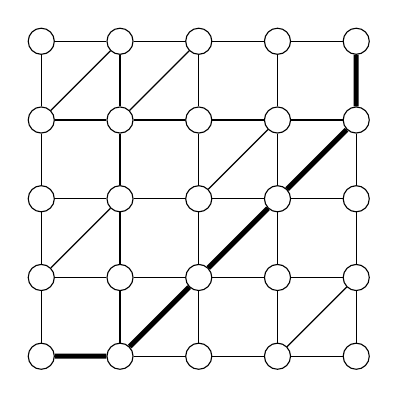
\begin{tikzpicture}
			\tikzstyle{every node}=[draw, shape=circle]
			\path (0,0) node (p00) {} 
			      (0,1) node (p01) {}
			      (0,2) node (p02) {}
			      (0,3) node (p03) {}
			      (0,4) node (p04) {}
			      (1,4) node (p14) {}
			      (1,3) node (p13) {}
			      (1,2) node (p12) {}
			      (1,1) node (p11) {}
			      (1,0) node (p10) {} 
			      (2,0) node (p20) {} 
			      (2,1) node (p21) {}
			      (2,2) node (p22) {}
			      (2,3) node (p23) {}
			      (2,4) node (p24) {}
			      (3,4) node (p34) {}
			      (3,3) node (p33) {}
			      (3,2) node (p32) {}
			      (3,1) node (p31) {}
			      (3,0) node (p30) {} 
			      (4,0) node (p40) {} 
			      (4,1) node (p41) {}
			      (4,2) node (p42) {}
			      (4,3) node (p43) {}
			      (4,4) node (p44) {};
			\draw (p00) -- (p10)
			      (p10) -- (p20)
			      (p20) -- (p30)
			      (p30) -- (p40);
			\draw (p01) -- (p11)
			      (p11) -- (p21)
			      (p21) -- (p31)
			      (p31) -- (p41);
			\draw (p02) -- (p12)
			      (p12) -- (p22)
			      (p22) -- (p32)
			      (p32) -- (p42);
			\draw (p03) -- (p13)
			      (p13) -- (p23)
			      (p23) -- (p33)
			      (p33) -- (p43);
			\draw (p04) -- (p14)
			      (p14) -- (p24)
			      (p24) -- (p34)
			      (p34) -- (p44);
			\draw (p00) -- (p01)
			      (p01) -- (p02)
			      (p02) -- (p03)
			      (p03) -- (p04);
			\draw (p10) -- (p11)
			      (p11) -- (p12)
			      (p12) -- (p13)
			      (p13) -- (p14);
			\draw (p20) -- (p21)
			      (p21) -- (p22)
			      (p22) -- (p23)
			      (p23) -- (p24);
			\draw (p30) -- (p31)
			      (p31) -- (p32)
			      (p32) -- (p33)
			      (p33) -- (p34);
			\draw (p40) -- (p41)
			      (p41) -- (p42)
			      (p42) -- (p43)
			      (p43) -- (p44);
			\draw (p01) -- (p12)
			      (p03) -- (p14)
			      (p10) -- (p21)
			      (p13) -- (p24)
			      (p21) -- (p32)
			      (p22) -- (p33)
			      (p30) -- (p41)
			      (p32) -- (p43);
			\draw[line width=1.8pt] (p00) -- (p10) -- (p21) -- (p32) -- (p43) -- (p44);
		\end{tikzpicture}
	\end{center}

	Now, it turns out that we can prove concentration results for this setting. In 
	particular, consider first the model where we let $X_{u,v}$ be the indicator of 
	whether the `cell' at co\"ordinates $(u,v)$ has a diagonal. Then, if $Z$ is the 
	random variable that takes as value the length of the shortest path between the 
	corners at $(0,0)$ and $(n,n)$, then clearly, $\exists f \in \{0,1\}^{n^2} 
	\rightarrow \mathbb{R}$ such that 
	$$
		Z = f \circ 
		\begin{bmatrix}
			X_{1,n} & \hdots & X_{n,n} \\
			\vdots & \ddots & \vdots \\
			X_{1,1} &\hdots & X_{n,1}
		\end{bmatrix}
	$$
	which is also Lipschitz with parameter $\mathbf{c} = (2-\sqrt 2) \mathbf{1}^{n\times n}$, 
	since taking away any diagonal means that the new shortest path is at most $2-\sqrt 2$ 
	units longer (by replacing the diagonal with one horizontal and one vertical grid-line),
	while adding any one diagonal would have (at best) the symmetrical effect of making the 
	path shorter. Consequently, combining the two bounds in McDiarmid's inequality, we get 
	$$
		\mathbb{P}(|Z-\mathbb{E}(Z)| \geq \epsilon) \leq 
		2 \exp \left(-\frac{2\epsilon^2}{(2-\sqrt 2)^2 n^2}\right).
	$$

	Interestingly, however, we may significantly improve on this bound by choosing the 
	variables of which we model $Z$ as a function differently. Suppose instead we consider 
	$Y_i = \begin{pmatrix} X_{i, 1} & \hdots & X_{i, n} \end{pmatrix}^T$, i.e.\ the $i$th column 
	of indicators of diagonals. Since any shortest path from $(0,0)$ to $(n,n)$ would comprise,
	at most, one diagonal from the $i$th column, again, there is a $g \in \left(\{0,1\}^{n}
	\right)^n \rightarrow \mathbb{R}$ such that 
	$$
		Z = g \circ \begin{bmatrix} Y_1 & \hdots & Y_n \end{bmatrix}
	$$
	that is Lipschitz with parameter $\mathbf{c}' = (2-\sqrt 2) \mathbf{1}^{n}$. Consequently,
	we can improve the above bound by the following, which is much tighter:
	$$
		\mathbb{P}(|Z-\mathbb{E}(Z)| \geq \epsilon) \leq 
		2 \exp \left(-\frac{2\epsilon^2}{(2-\sqrt 2)^2 n}\right).
	$$
	\ \\ \ \par
	Next, let us consider the example of the largest clique in an undirected graph. 
	Consider a graph $G = (V, E)$ drawn from the Erd\H{o}s-R\'enyi distribution with parameters
	$n,p$, and let $K$ be the largest integer such that $G$ has a complete subgraph of $K$
	vertices. Enumerating the possible edges in $G$ with $1 \hdots \binom{n}{2}$, and setting 
	$X_i$ to be the indicator of whether edge $i$ is present in $G$, we see that
	$$		
		\exists. f \in \{0,1\}^{\binom n 2} \rightarrow \mathbb{R} . 
		K = f \circ \begin{bmatrix} X_1 & \hdots & X_{\binom n 2 } \end{bmatrix}
	$$
	where, since each edge influences  the largest clique size by at most 1, $f$ is Lipschitz 
	with parameter $\mathbf{c} = \mathbf{1}^{\binom n 2}$, which leads us to conclude that 
	$$
		\mathbb{P}(|K - \mathbb{E}(K)| \geq \epsilon) \leq
		2 \exp\left(- \frac{2\epsilon^2}{\binom n 2}\right)
	$$
	However, we can again improve the bound. This follows from considering the variables
	$Y_i = \begin{pmatrix} 1[\{i,1\} \in E] & \hdots & 1[\{i, i-1\} \in E] \end{pmatrix}$,
	i.e.\ the collection of edges involving the $i$th vertex (and preceding other vertices).
	\ \\ \ \par
	As a final example, let us return to the Max-Cut problem we studied in the first chapter. 
	Consider a graph $G = (V,E)$ drawn from the Erd\H{o}s-R\'enyi model with parameters $n$ and 
	$\sfrac{1}{2}$, i.e.\ a graph having $n$ vertices in which each pari of vertices is 
	connected by an edge with probability $50\%$. Then, for some $S \subseteq V$, denote by 
	$E(S)$ the number of edges $\{u,v\} \in E$ such that $u \in S \land v \notin S$, the size 
	of the cut resulting from $S$. Note, then, that $\mathbb{E}(E(S)) = \frac{|S|(n-|S|)}{2} 
	\leq \sfrac{n^2}{8}$. Note also, that $E(S)$ is a function of each of the $|S|(n-|S|$ edges
	between $S$ and $V \setminus S$, which is Lipschitz with parameter $\mathbf{c} = 
	\mathbf{1}^{|S|(n-|S|)}$, meaning that
	$$
		\mathbb{P}(E(S) \geq (1+\delta)\mathbb{E}(E(S))) \leq 
		\exp\left(-\frac{2\delta^2\mathbb{E}(E(S))^2}{|S|(n-|S|)}\right).
	$$

	Then, we can deduce
	\begin{align*}
		& \mathbb{P}\left(E(S) \geq \sfrac{n^2}{8} + \delta \sfrac{n^2}{4}\right) \\
		&\leq \mathbb{P}\left(E(S) \geq (1+\sfrac{delta}{2})\mathbb{E}(E(S))\right) \\
		&\leq \exp\left(-\frac{\delta^2 \mathbb{E}(E(S))}{2|S|(n-|S|)}\right) \\
		&\in O\left(\exp\left(\delta^2n^2\right)\right)
	\end{align*}
	and by the union bound over all possible $S$, we have that
	$$
		\mathbb{P}\left(\exists S . E(S) \geq \sfrac{n^2}{8} + \sfrac{n^2}{4}\right) \in
		O\left(2^n\exp\left(\right)\right) = O\left(2^n\exp\left(c^2n\right)\right)
	$$
	where we pick $c = \delta \sqrt n$. Now, we can easily see that for $c$ large enough, 
	this means that, with high probability, the maximum cut in $G$ has size at most 
	$\sfrac{n^2}{8} + c\sqrt{n^3}$.
